\clearpage

\section{Trafik- och tumregler HF}
\subsection{Kort sammanfattning av reglemente}

OBS! Detta är inte fullständigt radioreglemente naturligtvis utan endast sammanfattning av några viktiga punkter.

\subsubsection{Begrepp i bandplanerna}

\begin{itemize}
\item QRP: Aktivitetscentrum för låg effekt ($<$5W), svaga signaler förekommer, visa hänsyn.
\item QRS: Aktivitetscenter för långsam CW.
\item QRSS: Extremt långsam CW med dator.
\item DV: Digital Voice.
\item Image: Bildmoder exempelvis SSTV och Fax som ryms inom den specificerade maximala bandbredden.
\end{itemize}

\subsubsection{Trafikregler och tumregler}

\begin{itemize}
\item Vid SSB-telefoni används LSB på frekvenser under 10 MHz och USB på frekvenser över 10 MHz.
\item Lägsta acceptabla inställda frekvens för LSB är 3 kHz över under bandkant! 
\item Högsta acceptable inställda frekvens för USB är 3 kHz under övre bandkant!
\item IBP är International Beacon Project. Fyrarna sänder med 3 min intervaller och används för att studera utbredningen av radiosignaler globalt. Fyrarna sänder anrop och fyra 1 s toner. Anropet och första tonen sänds med 100W, därefter sänds tonerna med 10W, 1W samt 100mW.
\item Vid AM (A3J) skall hänsyn tas så att störningar på annan trafik ej fö\-re\-kom\-mer med de sidband som då uppstår, det gäller då både övre och undre sidbandet.
\item Ingen som helst sändning är tillåtet inom fyrsegmenten. Detta skall respekteras. Lyssna gärna på nödfrekvenserna men används dem icke, om det inte är du som svarar på ett nödsamtal! Undvik QSO allt för nära dessa också.
\item Var särskilt uppmärksam på satelliters nerlänksfrekvenser på 10\,m-bandet. I detta segment skall endast lyssning ske. Ingen sändning är tillåten här eller i skyddssegmentet strax ovanför satellitsegmentet. Tänk på att satelliters frekvens kan dopplerskiftas uppåt en hel del när de rör sig mot mottagaren.
\end{itemize}

\section{Frekvenser HF}

\subsection{PR-bandet 27\,MHz}

Detta är det enda bandet som allmänheten kan använda på HF-bandet. Det delar många egenskaper med 31\,MHz jaktradiobandet men är ett band som är äldre och mer etablerat.

Maximal uteffekt på bandet är 4W RMS ERP dvs antennvinst överstigande en 1/2-vågs dipol (0 dBd, 2.12 dBi) måste inräknas i effekten efter avdrag för matningsförlust. Modulationsslag AM, FM och SSB (primärt används USB) är tillåtet på alla kanaler i dag. Traditionellt används kanal 24 för USB men i dag får vilken kanal som helst användas.

Kanalerna med A efter är upplåtna för radiostyrning och inte för telefoni. Undvik därför att använda dessa om du har en sändare som kan använda dessa frekvenser. De är med i tabellen för den skall vara komplett. 

\clearpage

\begin{longtable}{rrl|rrl}
	\textbf{Frekvens}& \textbf{Kanalnr}& \textbf{Övrigt}        
	& \textbf{Frekvens} & \textbf{Kanalnr} & \textbf{Övrigt}  \\
	\hline \endhead
	  26,965 &       1 &                &   27,215 &      21 &          \\
	  26,975 &       2 &                &   27,225 &      22 &          \\
	  26,985 &       3 &                &   27,255 &      23 &          \\
	  26,995 &      3A & Radiostyrning  &   27,235 &      24 & SSB      \\
	  27,005 &       4 &                &   27,245 &      25 &          \\
	  27,015 &       5 &                &   27,265 &      26 &          \\
	  27,025 &       6 &                &   27,275 &      27 &          \\
	  27,035 &       7 &                &   27,285 &      28 &          \\
	  27,045 &      7A & Radiostyrning  &   27,295 &      29 &          \\
	  27,055 &       8 &                &   27,305 &      30 &          \\
	  27,065 &       9 &                &   27,315 &      31 &          \\
	  27,075 &      10 &                &   27,325 &      32 &          \\
	  27,085 &      11 &                &   27,335 &      33 &          \\
	  27,095 &     11A & Tid. nödfrekv. &   27,345 &      34 &          \\
	  27,105 &      12 &                &   27,355 &      35 &          \\
	  27,115 &      13 &                &   27,365 &      36 &          \\
	  27,125 &      14 &                &   27,375 &      37 &          \\
	  27,135 &      15 &                &   27,385 &      38 &          \\
	  27,155 &      16 &                &   27,395 &      39 &          \\
	  27,165 &      17 &                &   27,405 &      40 &          \\
	  27,175 &      18 &                &          &         &          \\
	  27,185 &      19 &                &          &         &          \\
	  27,195 &     19A & Radiostyrning  &          &         &          \\
	  27,205 &      20 &                &          &         &        
\end{longtable}

Många apparater är endast FM i dag men det finns de som också har SSB. Äldre apparater hade oftast AM och FM och ibland även SSB. Telegrafi körs i princip inte på PR-bandet, troligen för att det aldrig varit några krav på det och de som kör heller inte haft möjlighet förr i tiden att DX-a på bandet. 

Innan Televerket släppte upp bestämmelserna var det väldigt hårda bestämmelser på bandet, i princip var det bara kommunikation inom familjen som tilläts. I dag kan bandet användas som man vill och det är på sina håll god aktivitet. 

Kom ihåg att inte överskrida effektbegränsningarna bara.

\subsection{JOTA---Jamboree on the air, scoutfrekvenser}

Scouterna har frekvenser på HF likväl som VHF/UHF som de aktiverar vid särskilda tillfällen ofta i tillsammans med en lokal amatörradioklubb eller vanliga amtörradioeldsjälar som inte sällan också är scouter. Här kommer en lista på frekvenser som är vanligt förekommande i scoutsammanhang.

\begin{table}[H]
\centering
\begin{tabular}{rrll}
	\textbf{Band} & \textbf{Frekvens} & \textbf{Trafik} & \textbf{Not} \\ \hline

               80 & 3 570  & CW  &             \\
	              & 3 940  & SSB & Ej region 2 \\
	              & 3 690  & SSB &             \\ \hline
	           40 & 7 030  & CW  &             \\
	              & 7 190  & SSB &             \\
	              & 7 090  & SSB &             \\ \hline
	           20 & 14 060 & CW  &             \\
	              & 14 290 & SSB &             \\ \hline
	           17 & 18 080 & CW  &             \\
	              & 18 140 & SSB &             \\ \hline
	           15 & 21 140 & CW  &             \\
	              & 21 360 & SSB &             \\ \hline
	           12 & 24 910 & CW  &             \\
	              & 24 960 & SSB &             \\ \hline
	           10 & 28 180 & CW  &             \\
	              & 28 390 & SSB &             \\ \hline
	            6 & 10 160 & CW  &             \\
	              & 50 160 & SSB &             \\ \hline
\end{tabular}
\caption{Scouters JOTA-frekvenser på HF}
\end{table}

Normalt aktiveras dessa frekvenser tredje veckoslutet i oktober varje år, fredag till söndag. Då kan det vara många klubbar som finns på frekvenserna och det är också vanligt att man hör dem på helt andra frekvenser. De frekvenser som listas här är inte på något vis de endra frekvenser som scouter använder.

\subsection{Marina MF/HF-frekvenser}

De marina HF-banden är uppdelade på ett antal band. Det finns en generell kanalindelning med 3 kHz per kanal och SSB som modulationssätt på respektive band. Marina HF-kanaler finns på banden 4, 6, 8, 12, 16, 18, 22 och 25 MHz. 

MF även benämnd gränsvåg i marina sammanahang är inte lika ofta används som den var en gång i tiden. Nedan listas de frekvenser som används i Sverige.

\subsubsection{Svenska MF-kanaler}

\begin{longtable}{llrr}
\textbf{Kanal} & \textbf{Placering} & \textbf{Skepp} & \textbf{Kust}  \\ \hline 
\endhead

MF1 & Gotland       & 2 099 & 1 6874 \\
MF2 & ---           & ---  & ---   \\
MF3 & Gislövshammar & 2 060 & 1 797  \\
MF4 & Härnösand     & 2 216 & 2 733  \\
MF5 & Bjuröklubb    & 2 123 & 1 779  \\
MF6 & Grimeton      & 2 135 & 1 710
\end{longtable}

\subsubsection{Nödfrekvenser}

\begin{longtable}{lrr}
\textbf{Band} & \textbf{Frekvens} & \textbf{DSC Frekvens}\\ \hline \endhead

MF   & 2 182  & 2 187.5  \\
HF4  & 4 125  & 4 207.5  \\
HF6  & 6 215  & 6 312.0  \\
HF8  & 8 291  & 8 414.5  \\
HF12 & 12 290 & 12 577.0 \\
HF16 & 16 429 & 16 804.5 \\
\end{longtable}

\subsubsection{Primära HF skepp-till-skepp}

\begin{longtable}{lrrrrrrrr}
\textbf{Kanal} & \textbf{HF4} & \textbf{HF6} & \textbf{HF8} & \textbf{HF12} & \textbf{HF16} & \textbf{HF18} & \textbf{HF22} & \textbf{HF25} \\
\hline
\endhead

A & 4 146 & 6 224 & 8 294 & 12 353 & 16 528 & 18 825 & 22 159 & 25 100 \\
B & 4 149 & 6 227 & 8 297 & 12 356 & 16 531 & 18 828 & 22 162 & 25 103 \\
C &       & 6 230 &       & 12 359 & 16 534 & 18 831 & 22 165 & 25 106 \\
D &       &       &       & 12 362 & 16 537 & 18 834 & 22 168 & 25 109 \\
E &       &       &       & 12 365 & 16 540 & 18 837 & 22 171 & 25 112 \\
F &       &       &       &        & 16 543 & 18 840 & 22 174 & 25 115 \\
G &       &       &       &        & 16 546 & 18 843 & 22 177 & 25 118 \\
\end{longtable}

\clearpage
\subsection{Fyrar}

\subsubsection{IBP -- International Beacon Project}

Det finns flera olika typer av fyrar men för HF är IBP (International Beacon Project) intressant eftersom det ger operatören möjlighet att utröna hur utbredningen ser ut för stunden genom att lyssna efter fyrar. Fyrarna har gemensam hårdvara och synkroniseras mot tidsreferens. Fyrar kan vara offline av olika skäl, kontrollera mot IBP:s hemsida om du inte hör en fyr du brukar höra.

Tabellen nedan visar anropssignaler och första sändningsslotten som fyren sänder, dvs SCHED för olika fyrar och frekvenser.

\subsubsection{Lista över IBP-fyrar}
\begin{table}[H]
\centering
\begin{tabular}{llrrrrr}
\textbf{Signal} & \textbf{QTH} & \textbf{14 100} & \textbf{18 110} & \textbf{21 150} & \textbf{24 930} & \textbf{28 200} \\ \hline

4U1UN  & United Nations & 00:00  & 00:10  & 00:20  & 00:30  & 00:40  \\ 
VE8AT  & Canada         & 00:10  & 00:20  & 00:30  & 00:40  & 00:50  \\
W6WX   & United States  & 00:20  & 00:30  & 00:40  & 00:50  & 01:00  \\
KH6RS  & Hawaii         & 00:30  & 00:40  & 00:50  & 01:00  & 01:10  \\
ZL6B   & New Zealand    & 00:40  & 00:50  & 01:00  & 01:10  & 01:20  \\
VK6RBP & Australia      & 00:50  & 01:00  & 01:10  & 01:20  & 01:30  \\
JA2IGY & Japan          & 01:00  & 01:10  & 01:20  & 01:30  & 01:40  \\
RR9O   & Russia         & 01:10  & 01:20  & 01:30  & 01:40  & 01:50  \\
VR2B   & Hong Kong      & 01:20  & 01:30  & 01:40  & 01:50  & 02:00  \\
4S7B   & Sri Lanka      & 01:30  & 01:40  & 01:50  & 02:00  & 02:10  \\
ZS6DN  & South Africa   & 01:40  & 01:50  & 02:00  & 02:10  & 02:20  \\
5Z4B   & Kenya          & 01:50  & 02:00  & 02:10  & 02:20  & 02:30  \\
4X6TU  & Israel         & 02:00  & 02:10  & 02:20  & 02:30  & 02:40  \\
OH2B   & Finland        & 02:10  & 02:20  & 02:30  & 02:40  & 02:50  \\
CS3B   & Madeira        & 02:20  & 02:30  & 02:40  & 02:50  & 00:00  \\
LU4AA  & Argentina      & 02:30  & 02:40  & 02:50  & 00:00  & 00:10  \\
OA4B   & Peru           & 02:40  & 02:50  & 00:00  & 00:10  & 00:20  \\
YV5B   & Venezuela      & 02:50  & 00:00  & 00:10  & 00:20  & 00:30  \\
\end{tabular}
\caption{IBP-fyrar}
\end{table}

\normalsize

\clearpage

\subsection{Olika trafiksätt på HF}

De olika HF-banden har olika egenskaper över tid på dagen, tid på året och påverkas vädligt mycket av rådande rymdväder och hur joniserat den övre delen av atmosfären är för att bilda rymdvåg.

Med det stora antalet band som radioamatörer förfogar över så finns det ofta något band som fungerar. Det gäller att man lär sig hur de olika egenskaperna påverkar de olika banden och när man kan förvänta sig att de ''öppnar'' och fungerar på längre avstånd.

Klassiska amatörradioband på kortvågen är därför 160 meter (som ju egentligen är ett gränsvågsband då det ligger precis under kortvågen enligt rådande ITU-definition), 80, 40, 60, 20, 17, 15, 12 och 10 metersbanden ger radioamatörer en stor karta av olika band att arbeta med.

För den som inte är radioamatör så är urvalet mer begränsat och även den effekt man lagligen får använda. Här finns egentligen bara 27~MHz och till nöds kan man väl även räkna jaktfrekvenserna på 31~MHz också men begränsningen i användandet och vilken effekt som står till buds gör att kortvågen är radioamatörernas jaktmark i första hand.

Vi ska i det här kapitlet titta lite på de olika bandens olika egenskaper och lite olika sätt att använda dem för att nå lokalt, lite längre och DX -- dvs i det närmaste globalt.

\subsubsection{Solens inverkan -- rymdvädret}

En sak som har mycket kraftig inverkan på radiosamband på kortvåg är rymdvädret. Som många känner till så följer solens solfläckar en 11-årig cykel och just nu inväntar vi toppen på cykel nummer 25 (numrerad från 1 sedan man började numrera dem) och dess topp förväntas inträffa under 2025. Därefter kommer vi se en nedgång i solfläckar fram till början av nästa cykel, som då blir cykel 26. 

I botten på solfläckscyklerna blir det ofta sämre så kallade konditioner på kortvågsbanden. Det blir svårare att nå långt och hitta ''öppningar'' på banden med högre frekvens, framför allt 15-, 12- och 10-metersbanden. Lokalt fungerar de bra men för de där riktiga DX-öppningarna behövs lite solaktivitet.

I toppen på solcykeln kan det däremot vara väldigt varierande. Ena dagen har man enorma öppningar på 10-metersbandet så att man kan kommunicera lokalt, men risken för en kraftig så kallad ''flare'' från solen eller en CME (koronal mass-utkasning, Coronal Mass Ejection) där en del av solens yta slungas iväg i kraftiga explosioner påverkar inte bara solvindens möjligheter att jonisera de övre luftlagren utan kan också skapa störningar i det jordmagnetiska fältet.

När detta sker brukar det åtföljas av kraftiga och vackra polarsken (norrksen i norr och sydsken i syd) och amatörerna benämner dessa som ''aurora''. Då denna uppträder är ofta kortvågen kraftigt påverkad på ett negativt sätt men ibland kan man nyttja själva auroran och studsa lite högre frekvenser på den som t.ex. VHF och då exempelvis 6-metersbandet eller 2-metersbandet.

\subsubsection{Markvåg}

Precis som för VHF och UHF så finns det på kortvåg också en markvåg. Den är dock relativt begränsad i sin utbredning och kommer något längre än den sträcka man kan beräkna med formler för VHF, dvs radiohorisonten. Kortvåg har en förmåga att ta sig en smula längre i alla fall men främst är det rymdvågsegenskaperna som är den intressanta.

\subsubsection{Rymdvåg}

Rymdvågen är den utbrednignsform som gör kortvåg till ett globalt kommunikationsmedel. Genom att den övre delen av atmosfären joinseras av solens strålning -- jonosfären -- så kommer också radiovågor under en viss frekvens att kunna studsa mot dessa.

Denna frekvens kallas för MUF (maximum useable frequency) och betyder i praktiken den högsta frekvensen som fortfarande reflekteras i jonosfären. Frekvenser under MUF går också att använda men frekvenser över MUF fungerar mycket dåligt.

På olika ställen runt jorden mäts MUF genom så kallade ''jonosonder'' som innebär att man skickar en svept signal, ofta från ca 2~MHz till ungefär 40~MHz och sedan lyssnar man på olika mottagarstationer vad som kommer tillbaka och hur starkt det är. På amatörradions mottagare kan man ibland höra ett sådant svep och då är det reflexten av jonosonden som man hör.

\subsubsection{Generellt om kortvågbandens rymdvåg}

Lägre frekvenser reflekteras oftast på lägre nivå i jonosfären, de tränger inte lika högt upp i de olika reflekterande lagren innan de reflekteras. På samma sätt reflekteras i regel högre frekvenser högre upp. Detta gör att givet en viss vinkel så kommer den reflekterade rymdvågen ner på olika ställen, olika långt bort från sändaren, beroende på frekvensen. 

För att komma så långt som möjligt bör man välja ett band som är så nära MUF som möjligt och ha en relativt flack vinkel från sin antenn. För att uppnå NVIS skickar man signalen med en brant vinkel, nästan vertikalt uppåt, och den kommer då tillbaka ganska rakt uppifrån.

\subsubsection{NVIS}

Ett särskilt sätt att sända kortvåg är att skicka signalen nästan rakt uppåt. Sättet kallas på engelska för ''Near Vertical Incidence Skywave'' och kan översättas ungefär som ''nästan vertikalt vinklad rymdvåg'' och innebär att man placerar en kortvågsantenn relativt lågt, ibland bara några meter över mark. Man får då en våg som riktas i det närmaste rakt uppåt då marken agerar som en mycket nära reflektor.

Denna typ av rymdvåg träffar då de joniserade delarna av atmosfären och reflekteras tillbaka till marka, man kan beskriva det ungefär som ett ''paraply'' av signaler som kommer ner. Radien är ofta mellan 400--600~km vilket gör att man kan täcka in en stor del av skandinavien och norra Europa med NVIS.

Lämpliga band för NVIS är band mellan 2--8 MHz så för oss radioamatörer blir det då 160-, 80-, 40-metersbanden främst, men även 60-metersbandet kan nyttjas för NVIS.

%\begin{figure}[h]
%	\centering
%	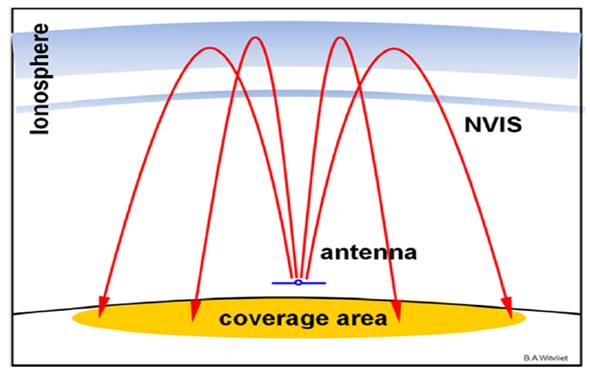
\includegraphics[width=0.6\textwidth]{bilder/NVIS-Propagation}
%	\label{fig:nvis-propagation}
%	\caption{NVIS-utbredning, princip}
%\end{figure}

NVIS används mycket på t.ex. 80-metersbandet för olika ''ringar'' och liknande när man träffas flera sändaramatörer på en viss frekvens en viss tid och sedan turas om att sända och kommentera på olika saker. 

\subsubsection{DX -- långväga kontakter}

För mer långväga kontakter lägger vi oss så högt det går, har antenner som sänder i en flackare vinkel, nästan rakt mot horisonten på lite högre höjd om möjligt och gärna också riktantenner i stället för de vanliga dipolerna som är den vanligaste antennen för de lägre kortvågsbanden.

Genom att kombinera detta och reflektera så högt upp i jonosfären som möjligt kan vi ibland nå mycket långt. Är konditionerna goda kan man få flera sådana hopp (skip) efter varandra och på så vis kan vi nå till andra sidan planeten. Vid gynnsamma konditioner kan man med relativt enkla medel prata med Japan och Australien på kortvåg.

\subsection{Bandens olika egenskaper}

\todo{Beskriva}

\subsubsection{160--80 meter}
\todo{Beskriva}


\subsubsection{40-60 meter}
\todo{Beskriva}

\subsubsection{20, 17, 12 och 10 meter}
\todo{Beskriva}



\begin{landscape}
\section{Frekvenser Amatörradio LF/MF/HF}
\subsection{Bandplaner LF/MF/HF}
Alla frekvenser i kHz, bandbredder i Hz.

\subsubsection{Bandplan 2.2\,km, 135,7--137,8\,kHz}
\begin{tabular}{rrrll}
\textbf{Frekvens} &  & \textbf{BW} & \textbf{Trafik} & \textbf{Noteringar} \\ \hline
135,7 & 135,8 & 200 & CQ, QRSS, Digi & OBS! Högsta effekt 1W ERP. \\ \hline
\end{tabular}

\subsubsection{Bandplan 600\,m, 472--479\,kHz}
\begin{tabular}{rrrll}
\multicolumn{2}{c}{\textbf{Frekvens}} & \textbf{BW} & \textbf{Trafik} & \textbf{Noteringar} \\ \hline
472 & 479 & 200 & CW, QRSS, Digi & OBS! Högsta utstrålad effekt 1W EIRP \\ \hline
\end{tabular}

\subsubsection{Bandplan 160\,m, 1810--2000\,kHz}
\begin{tabular}{rrrll}
\multicolumn{2}{c}{\textbf{Frekvens}} & \textbf{BW} & \textbf{Trafik} & \textbf{Noteringar} \\ \hline
1 810 & 1 838 & 200  & CW         & Exklusivt för CW. Interkontinental trafik har prio. \\ \hline
1 838 & 1 840 & 500  & Smalband   & Ej packet på 160m, PSK 1 838,150                    \\ \hline
1 840 & 1 850 & 2700 & Alla moder & Även digimode. SSB QRP 1 843 kHz                    \\ \hline
1 850 & 1 900 & 2700 & Alla moder & OBS! Max 10 W till ant.                             \\ \hline
1 900 & 1 950 & 2700 & Alla moder & OBS! Max 100 W till ant.                            \\ \hline
1 950 & 2 000 & 2700 & Alla moder & OBS! Max 10 W till ant.                             \\ \hline
\end{tabular}

\subsubsection{Bandplan 80\,m, 3500--3800\,kHz}
\begin{tabular}{rrrll}
\multicolumn{2}{c}{\textbf{Frekvens}} & \textbf{BW} & \textbf{Trafik} & \textbf{Noteringar} \\ \hline
3 500 & 3 510 & 200  & CW             & Exklusivt CW                         \\ 
      &       &      &                & Interkontinental DX-trafik har prio  \\ \hline
3 510 & 3 580 & 200  & CW             & Exklusivt CW contest 3510-–560       \\ 
      &       &      &                & CW QRS 3 555 kHz, CW QRP 3 560       \\ \hline
3 580 & 3 600 & 500  & Smalband, Digi & PSK 3 580,150                        \\
      &       &      &                & Automatiska Digimoder 3 590--600     \\ \hline
3 600 & 3 620 & 2700 & Alla moder     & Digimoder Automatiska Digimoder      \\ \hline
3 600 & 3 650 & 2700 & Alla moder     & SSB contest 3 600--650               \\
      &       &      &                & DV 3 630                             \\ \hline
3 650 & 3 700 & 2700 & Alla moder     & SSB QRP 3 690                        \\ \hline
3 700 & 3 800 & 2700 & Alla moder     & Contest 3 700-–800                   \\
      &       &      &                & Image 3 775                          \\
      &       &      &                & Region 1 nödfrekvens 3 760           \\ \hline
3 775 & 3 800 & 2700 & Alla moder     & Interkontinental DX-trafik prioritet \\ \hline
\end{tabular}

\subsubsection{Bandplan 40\,m, 7000--7200\,kHz}
\begin{tabular}{rrrll}
\multicolumn{2}{c}{\textbf{Frekvens}} & \textbf{BW} & \textbf{Trafik} & \textbf{Noteringar} \\ \hline
7\,000 & 7\,040 & 200  & CW         & Exklusivt CW.                             \\
      &       &      &            & QRP aktivitetscentrum 7\,030\,kHz           \\ \hline
7\,040 & 7\,050 & 500  & Smalband   & Digimoder Automatiska inom 7\,047–-050\,kHz \\ \hline
7\,050 & 7\,060 & 2700 & Alla moder & Digimoder Automatiska inom 7\,050–-053\,kHz \\ \hline
7\,060 & 7\,100 & 2700 & Alla moder & SSB contest i segmentet                   \\
      &       &      &            & DV 7 070 kHz, SSB QRP 7\,090 kHz           \\ \hline
7\,100 & 7\,130 & 2700 & Alla moder & Region 1 nödfrekvens 7\,110 kHz            \\ \hline
7\,130 & 7\,200 & 2700 & Alla moder & SSB contest i segmentet                   \\
      &       &      &            & Image 7\,165\,kHz                           \\ \hline
7\,175 & 7\,200 & 2700 & Alla moder & Interkontinental DX-trafik prio           \\ \hline
\end{tabular}

\subsubsection{Bandplan 30 m, 10100--10150 kHz}
\begin{tabular}{rrrll}
\multicolumn{2}{c}{\textbf{Frekvens}} & \textbf{BW} & \textbf{Trafik} & \textbf{Noteringar} \\ \hline
10\,100 & 10\,140 & 200 & CW       & CW exkl. Max 150 Watt på 30 m    \\
       &        &     &          & CW QRP 10\,116\,kHz                     \\ \hline
10\,140 & 10\,150 & 500 & Smalband & Digimoder PSK 10142,150\,kHz. Ej Packet \\ \hline
\end{tabular}

\subsubsection{Bandplan 20 m, 14000--14350 kHz}
\begin{tabular}{rrrll}
\multicolumn{2}{c}{\textbf{Frekvens}} & \textbf{BW} & \textbf{Trafik} & \textbf{Noteringar} \\ \hline
14\,000 & 14\,070 & 200  & CW         & Exklusivt CW                            \\
       &        &      &            & Conctest 14\,000-–060                     \\
       &        &      &            & CW QRS 14 055, CW QRP 14\,060            \\ \hline
14\,070 & 14\,099 & 500  & Smalband   & PSK 14 070,150                          \\
       &        &      &            & Auto Digimoder 14 089-–099              \\ \hline
14\,099 & 14\,101 & 200  & Fyrar      & Exklusivt IBP, endast fyrar             \\ \hline
14\,101 & 14 \,12 & 2700 & Alla moder & Digitala moder och obevakade Digimoder  \\ \hline
14\,112 & 14\,350 & 2700 & Alla moder & SSB Contest 14 125--300                 \\
       &        &      &            & DV 14 130, DXpedition prio 14\,195$\pm$5 \\ \hline
14\,300 & 14\,350 & 2700 & Alla moder & Image 14\,230, SSB QRP 14\,285            \\
       &        &      &            & Global nödfrekvens 14 300               \\ \hline
\end{tabular}

\subsubsection{Bandplan 17 m, 18068--18168 kHz}
\begin{tabular}{rrrll}
\multicolumn{2}{c}{\textbf{Frekvens}} & \textbf{BW} & \textbf{Trafik} & \textbf{Noteringar} \\ \hline
18 068 & 18 095 & 200  & CW         & CW exklusivt. QRP 18 086             \\ \hline
18 095 & 18 109 & 500  & Smalband   & Digimoder PSK 18 100,150             \\
       &        &      &            & Automatiska Digimoder 18 105-–18 109 \\ \hline
18 109 & 18 111 & 200  & Fyrar      & Exklusivt fyrar, IBP fyrnät          \\ \hline
18 111 & 18 168 & 2700 & Alla moder & Digi 18 111–-18 120                  \\
       &        &      &            & SSB QRP 18 130, DV 18 150            \\
       &        &      &            & Global nödfrekv. 18 160\\ \hline
\end{tabular}

\subsubsection{Bandplan 15 m, 21000--21450 kHz}
\begin{tabular}{rrrll}
\multicolumn{2}{c}{\textbf{Frekvens}} & \textbf{BW} & \textbf{Trafik} & \textbf{Noteringar} \\ \hline
21 000 & 21 070 & 200  & CW         & Exklusivt CW, QRS 21 055, CW QRP 21 060          \\ \hline
21 070 & 21 110 & 500  & Smalband   & PSK 21080.150, Automatiska Digimoder 21 090–-110 \\
21 110 & 21 120 & 2700 & Alla moder & Alla moder utom SSB!                             \\
       &        &      &            & Digimoder, och Automatiska Digimoder             \\ \hline
21 120 & 21 149 & 500  & Smalband   &                                                  \\ \hline
21 149 & 21 151 & 200  & Fyrar      & Exklusivt fyrar. IBP fyrnät                      \\ \hline
21 151 & 21 450 & 2700 & Alla moder & DV 21 180, SSB QRP 21 285, Image 21 340          \\
       &        &      &            & Global nödfrekv. 21 360                          \\ \hline
\end{tabular}

\subsubsection{Bandplan 12 m, 24890--24990 kHz}
\begin{tabular}{rrrll}
\multicolumn{2}{c}{\textbf{Frekvens}} & \textbf{BW} & \textbf{Trafik} & \textbf{Noteringar} \\ \hline
24 890 & 24 915 & 200  & CW         & Exklusivt CW, QRP 24 906                             \\ \hline
24 915 & 24 929 & 500  & Smalband   & PSK 24 920.150, Automatiska Digimoder 24 925–-24 929 \\ \hline
24 929 & 24 931 & 200  & Fyrar      & Fyrar, IBP fyrnät                                    \\ \hline
24 931 & 24 990 & 2700 & Alla moder & Auto Digimoder 24 931-–24 940                        \\
       &        &      &            & SSB QRP 24 950, DV 24 960                            \\ \hline
\end{tabular}

\subsubsection{Bandplan 10 m, 28000-29700 kHz}
\begin{tabular}{rrrll}
\multicolumn{2}{c}{\textbf{Frekvens}} & \textbf{BW} & \textbf{Trafik} & \textbf{Noteringar} \\ \hline
28 000 & 28 070 & 200  & CW         & Exklusivt CW, QRS 28 055, CW QRP 28 060                \\ \hline
28 070 & 28 190 & 500  & Smalband   & PSK 28 120.150, Auto Digimoder inom 28 120--150        \\ \hline
28 190 & 28 199 & 200  & Fyrar IBP  & Regionala fyrar med tidsdelning                        \\ \hline
28 199 & 28 201 & 200  & Fyrar IBP  & IBP fyrnät                                             \\ \hline
28 201 & 28 225 & 200  & Fyrar IBP  & kontinuerligt sändande fyrar                           \\ \hline
28 225 & 28 300 & 2700 & Alla moder & Övriga fyrar                                           \\ \hline
28 300 & 28 320 & 2700 & Alla moder & Digimoder och Automatiska Digimoder                    \\ \hline
28 320 & 29 100 & 2700 & Alla moder & DV 28 330 kHz, SSB QRP 28 360 kHz                      \\
       &        &      &            & Image 28 680 kHz                                       \\ \hline
29 100 & 29 200 & 6000 & Alla moder & FM simplex, 10 kHz kanaler                             \\
       &        &      &            & Maximalt ±2.5 kHz dev., max 2.5 kHz mod.frek.          \\ \hline
29 200 & 29 300 & 6000 & Alla moder & Digimoder och Automatiska Digimoder                    \\ \hline
29 300 & 29 510 & 6000 & Satellit   & Nerlänk fr. satellit. EJ SÄNDNING I SEGMENTET          \\ \hline
29 510 & 29 520 & 6000 & Skydd      & Skyddsfrekvens för satelliter. EJ SÄNDNING I SEGMENTET \\ \hline
29 520 & 29 590 & 6000 & Alla moder & FM Repeater in RH1--8, 100 kHz duplex, 2.5 kHz NBFM    \\ \hline
29 600 & 29 620 & 6000 & Alla moder & FM simplex, anrop 29 600                               \\
       &        &      &            & FM simplex repeater 29 610                             \\ \hline
29 620 & 29 700 & 6000 & Alla moder & FM Repeater ut RH1--8, 100 kHz duplex                  \\ \hline
\end{tabular}
\end{landscape}

\clearpage

